\documentclass[8pt, letterpaper]{article}
\usepackage[ngerman]{babel}
\usepackage{graphicx}
\usepackage[utf8]{inputenc}
\usepackage{gensymb}
\usepackage{blindtext}
\usepackage{geometry}
\usepackage{fancyhdr}
\usepackage{url}
\usepackage{seqsplit}
\usepackage{hyperref}

\graphicspath{{images/}}
\setlength{\parindent}{0cm}
\bibliographystyle{gerplain}
\geometry{letterpaper, margin=2cm}
\pagestyle{fancy}

\lhead{Jakob Kirsch}
\rhead{
\includegraphics[width=3cm]{logo}}

\title{}
\author{Jakob Kirsch}
\date{\parbox{\linewidth}{\centering%
  \today\endgraf\bigskip
  Fach: IT\endgraf\medskip
  Betreür: Herr Kutzner\endgraf\medskip
}}

\begin{document}

\maketitle
\newpage

\section{Aufgabenstellung}
Es sollen die Stromstärke und Spannung eines Arduino UNOs und eventuelle Peripherien gemessen werden, um deren Verbrauch zu messen.
Uns wurden 4 verschiedene Szenarien gegeben:

\begin{enumerate}
  \item Im laufenden Betrieb ohne zusätzliche Bauteile
  \item Im laufenden Betrieb mit einer leuchtenden roten LED
  \item Im laufenden Betrieb mit einer leuchtenden blauen LED
  \item Im laufenden Betrieb mit einem Servomotor in ständiger Bewegung
\end{enumerate}

\section{Versuchsmaterial}
\begin{itemize}
  \item Arduino UNO
  \item Breadboard
  \item diverse Kabel für das Breadboard und den Arduino UNO
  \item 9V Batterie
  \item Digitalmultimeter
  \item Klemmen für das Digitalmultimeter
  \item Widerstände für die LEDs
  \item rote LED
  \item blaue LED
  \item Servomotor
\end{itemize}

\section{Messchaltungen}
\subsection{Spannungsmessung}
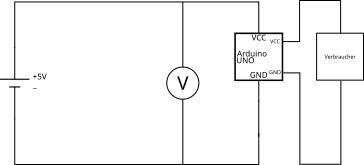
\includegraphics[width=9cm]{volt}
\subsection{Stromstärkemessung}
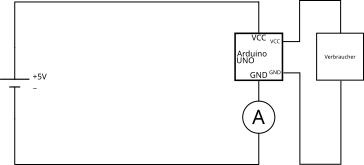
\includegraphics[width=9cm]{ampere}

Dabei sind die Verbrauchergruppen:
\begin{enumerate}
  \item Nichts
  \item Eine rote LED und ein Widerstand (1 \(k\Omega\))
  \item Eine blaue LED und ein Widerstand (1 \(k\Omega\))
  \item Ein Servomotor, welcher zusätzlich an einem weiteren Pin des Arduinos angeschlossen ist
\end{enumerate}

Die Stromquelle ist eine 9V Batterie, damit man nicht bei einem falschen Aufbau den PC beschädigt.

\subsection{Bilder}
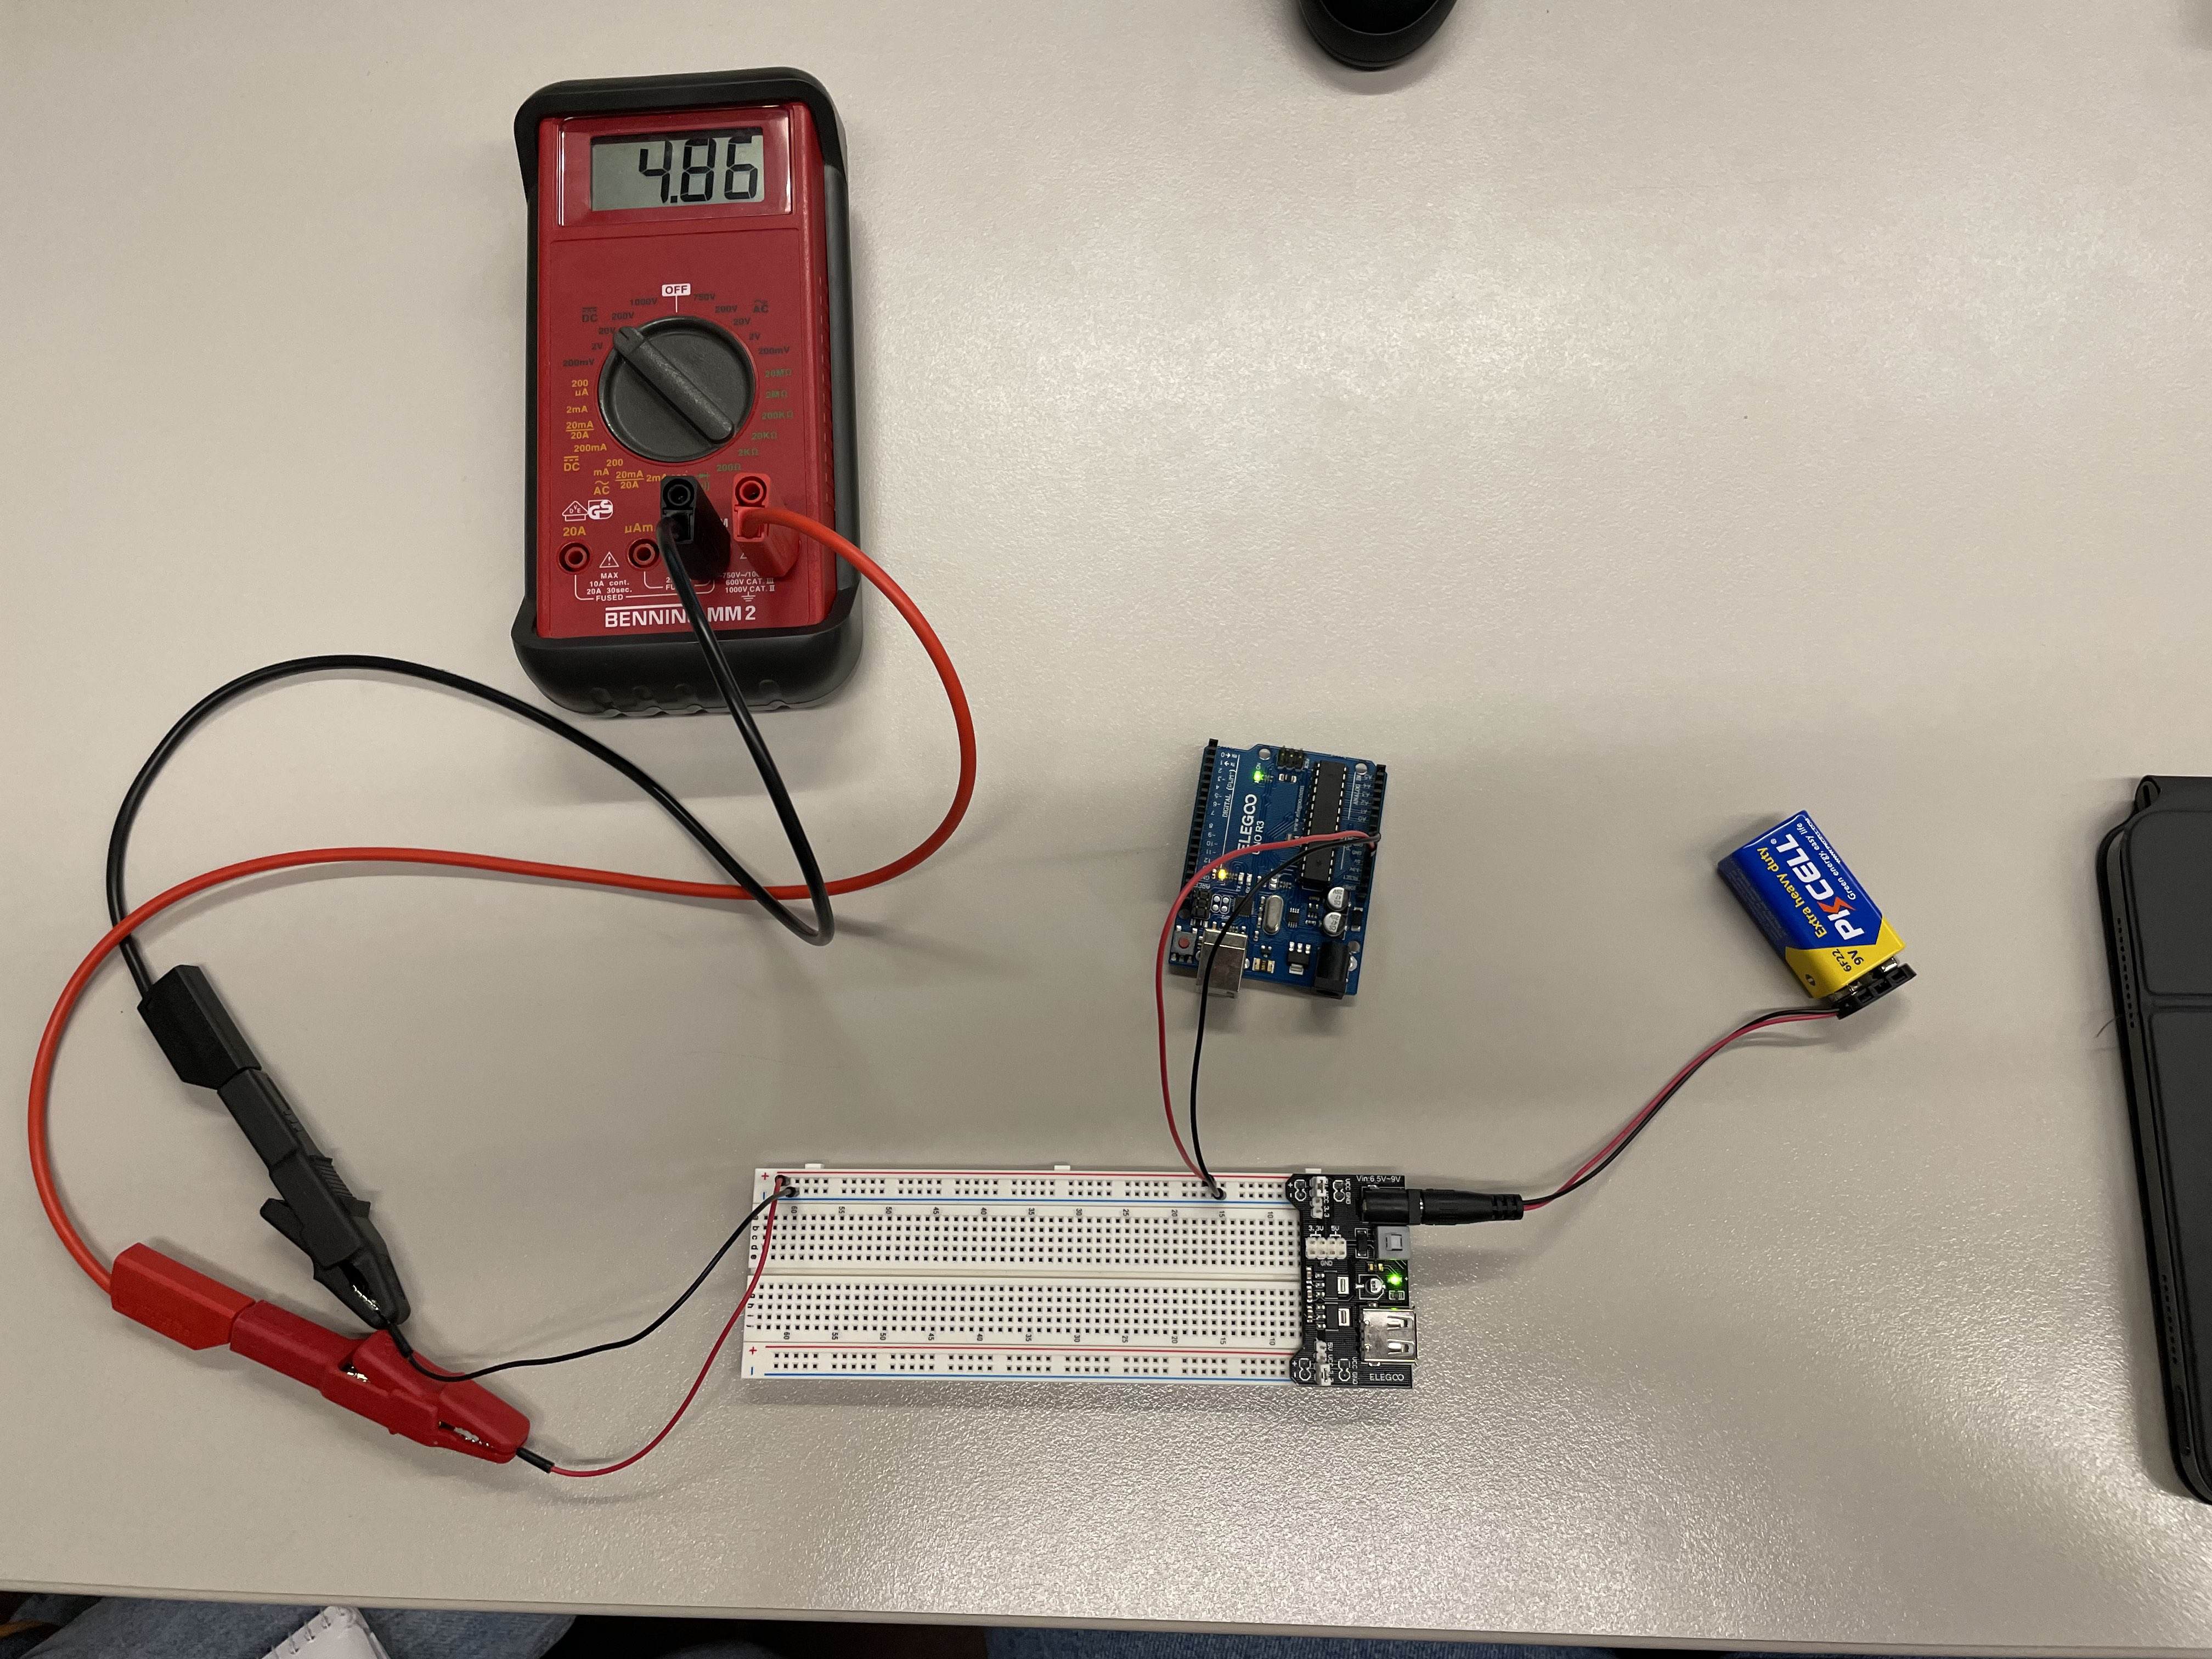
\includegraphics[width=9cm]{aufbau1}
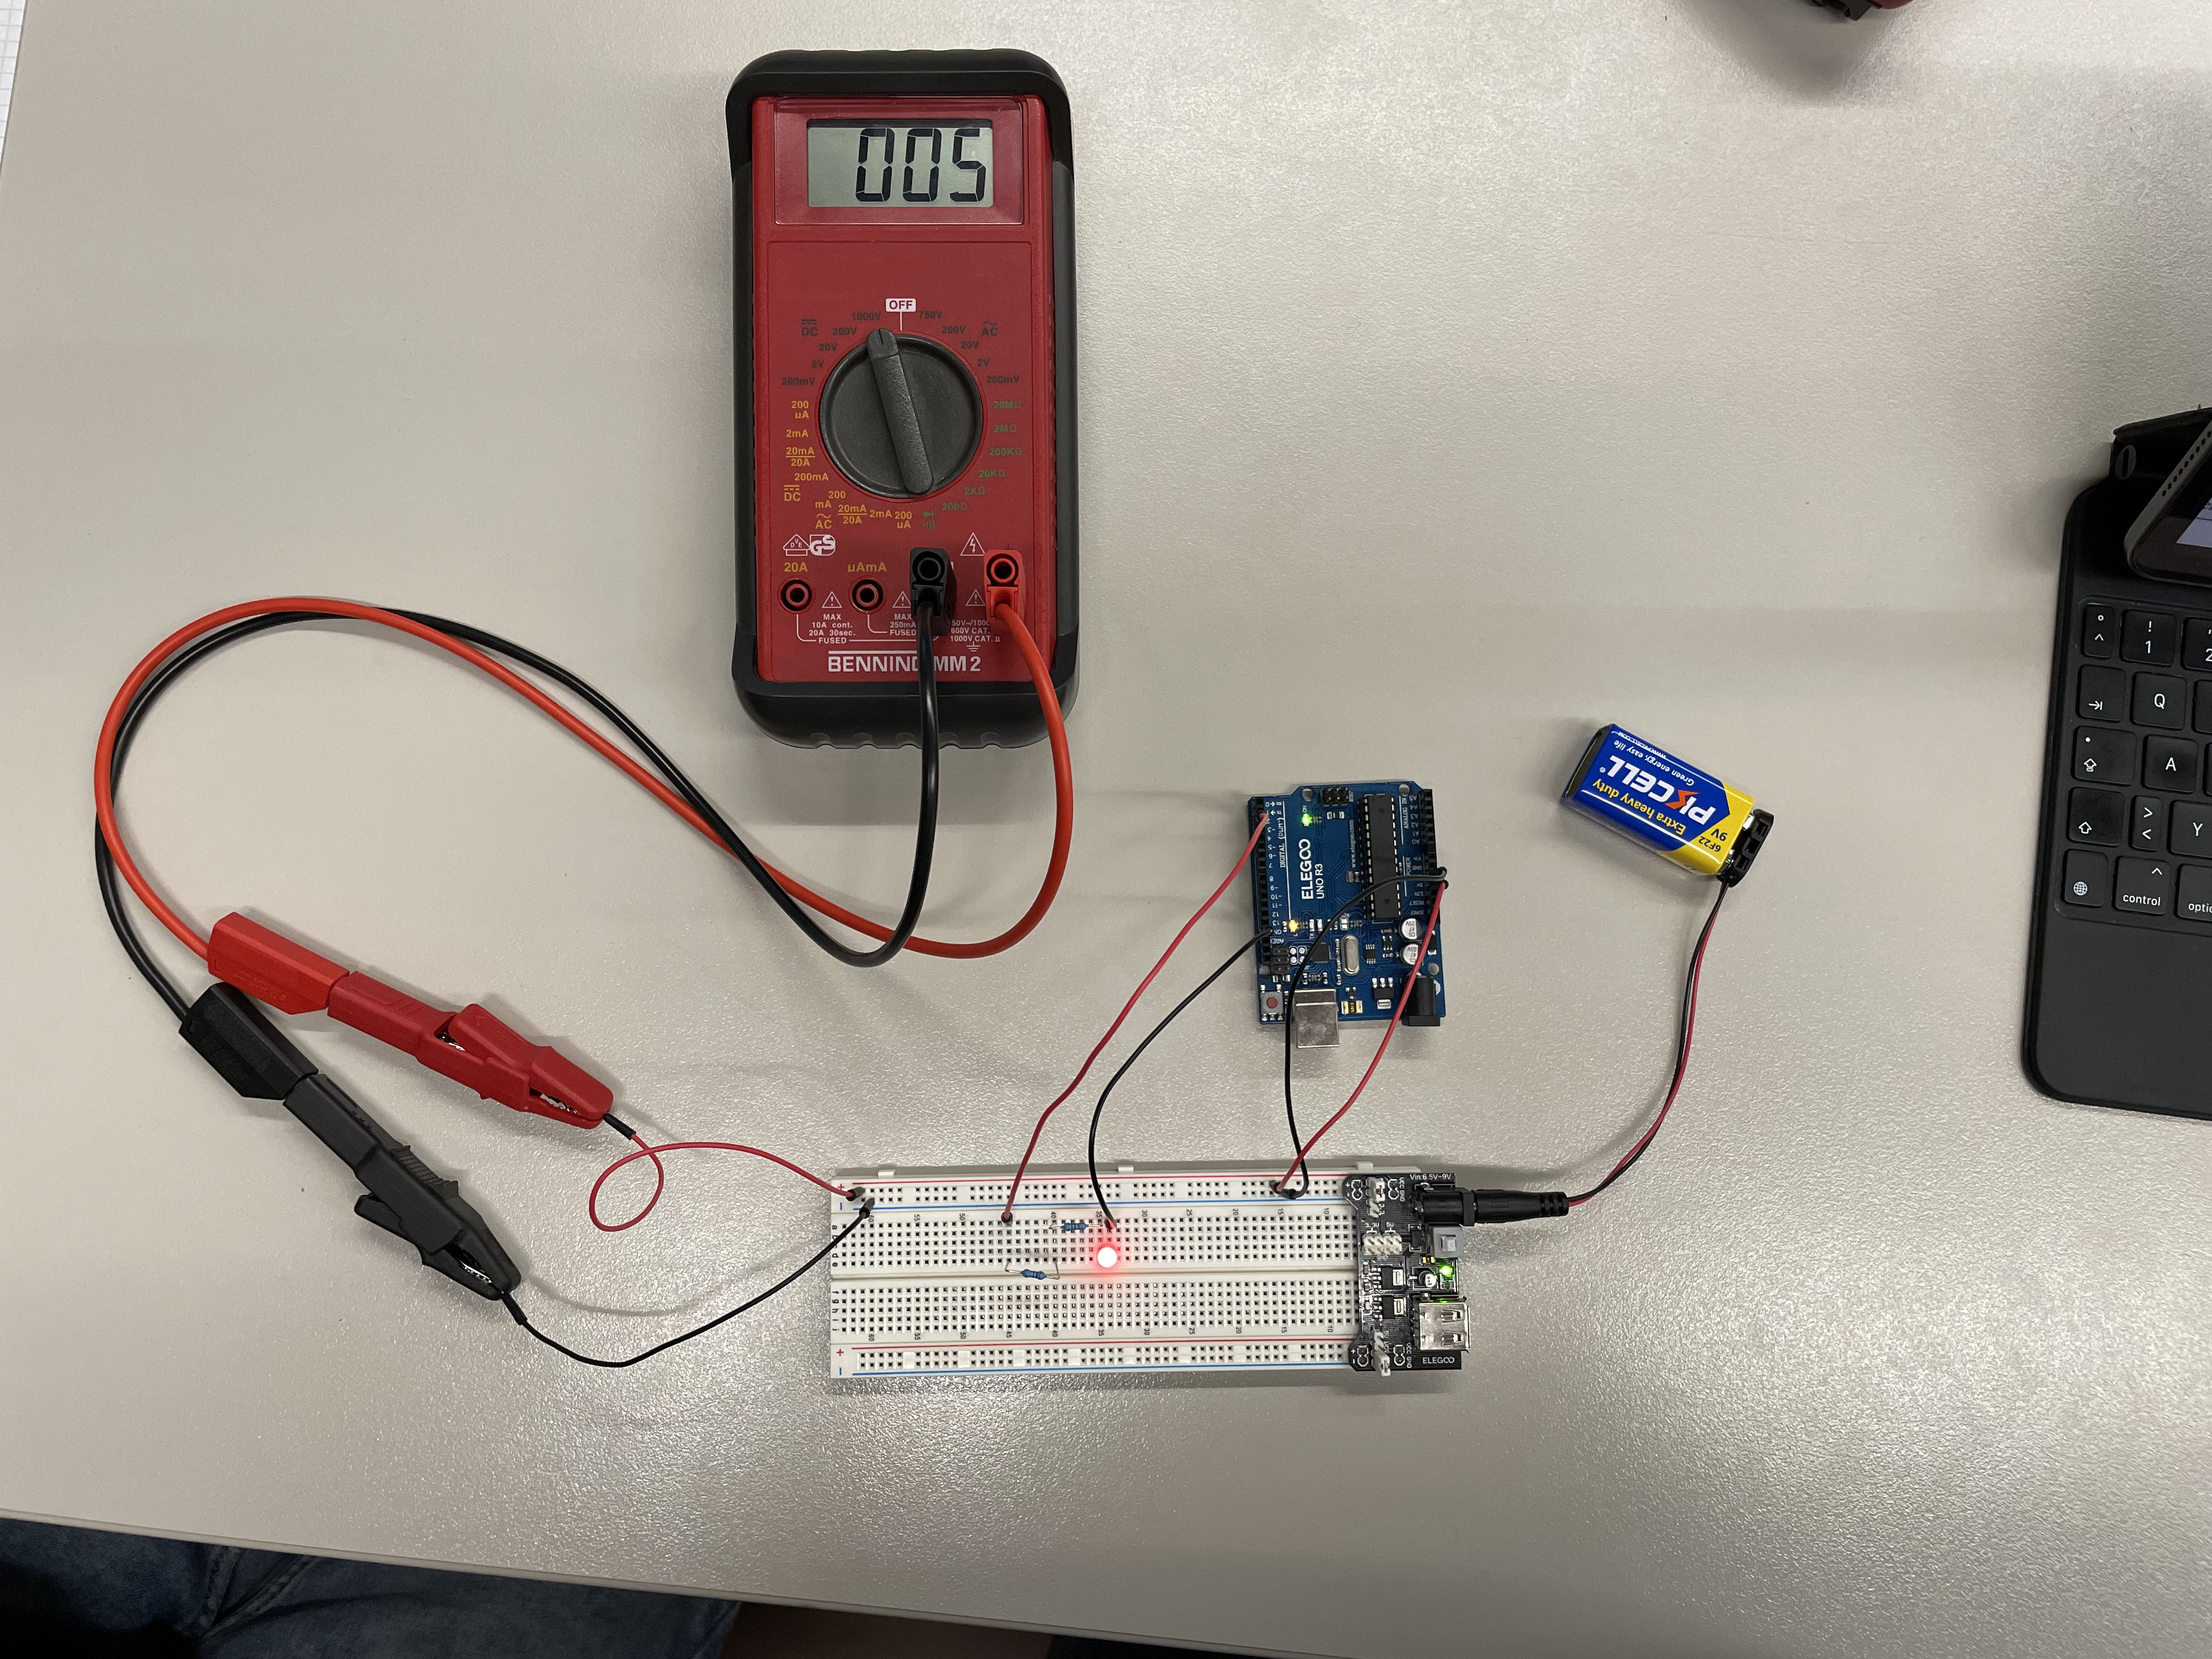
\includegraphics[width=9cm]{aufbau2}
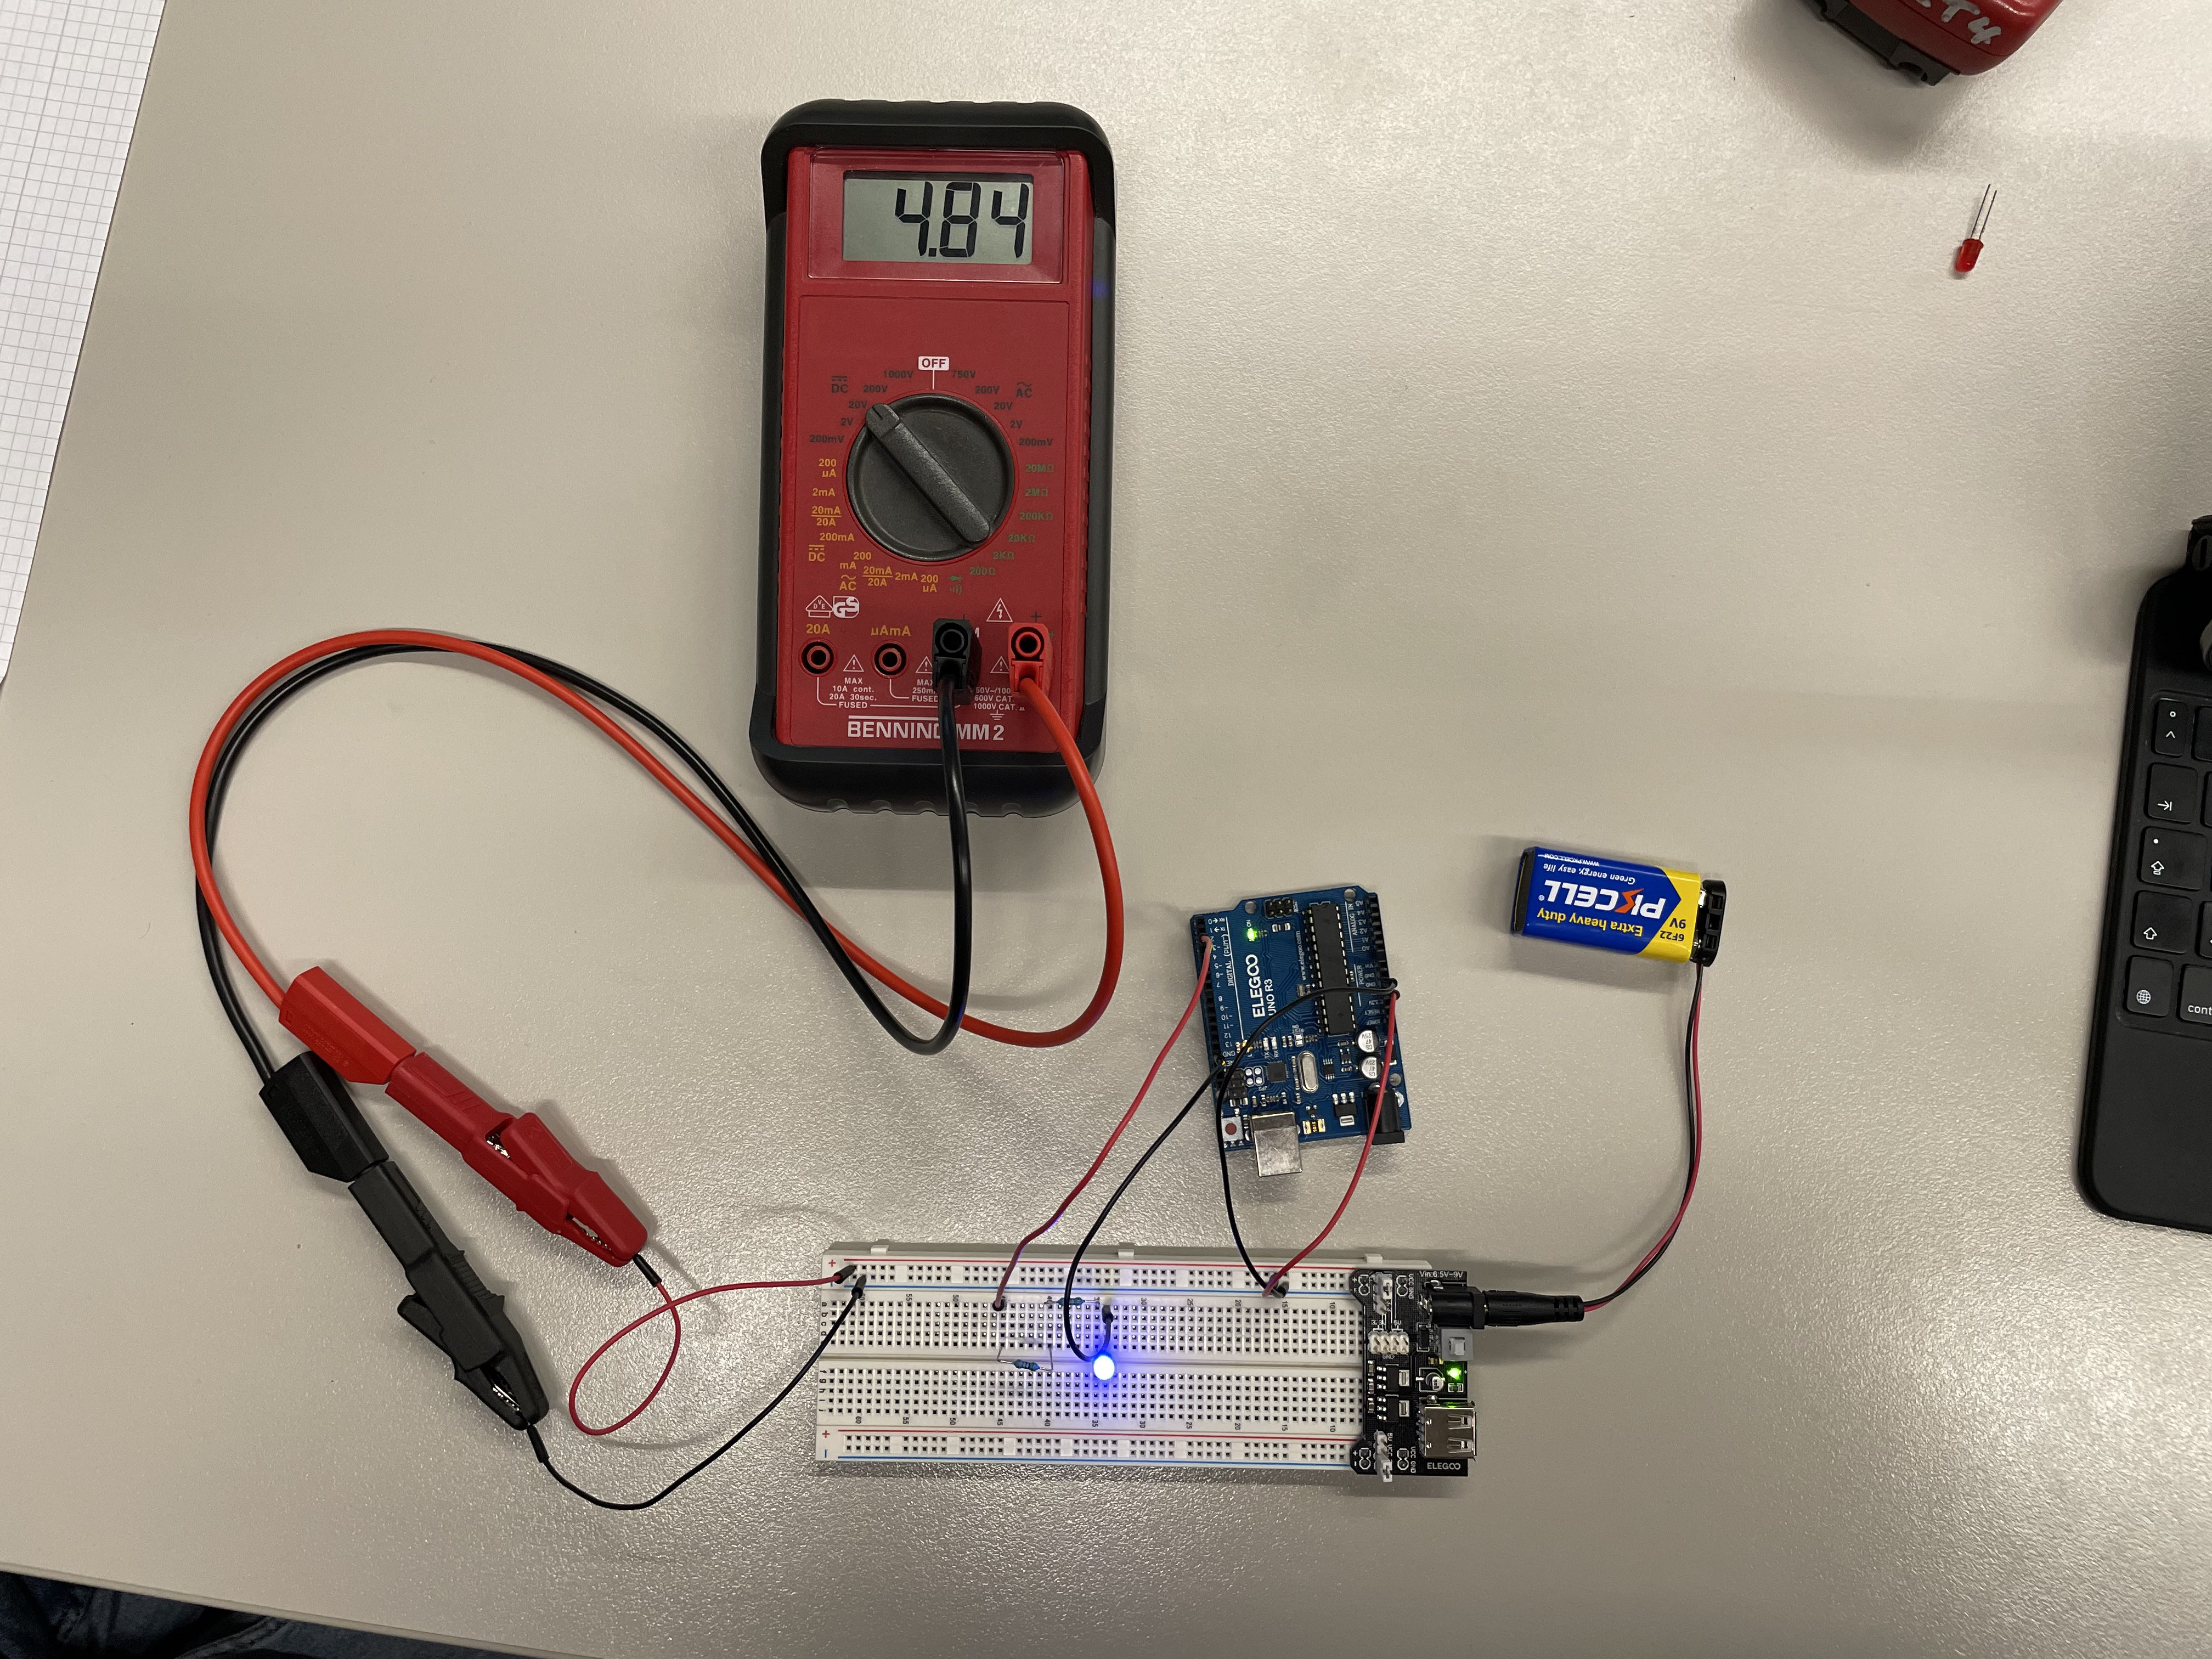
\includegraphics[width=9cm]{aufbau3}
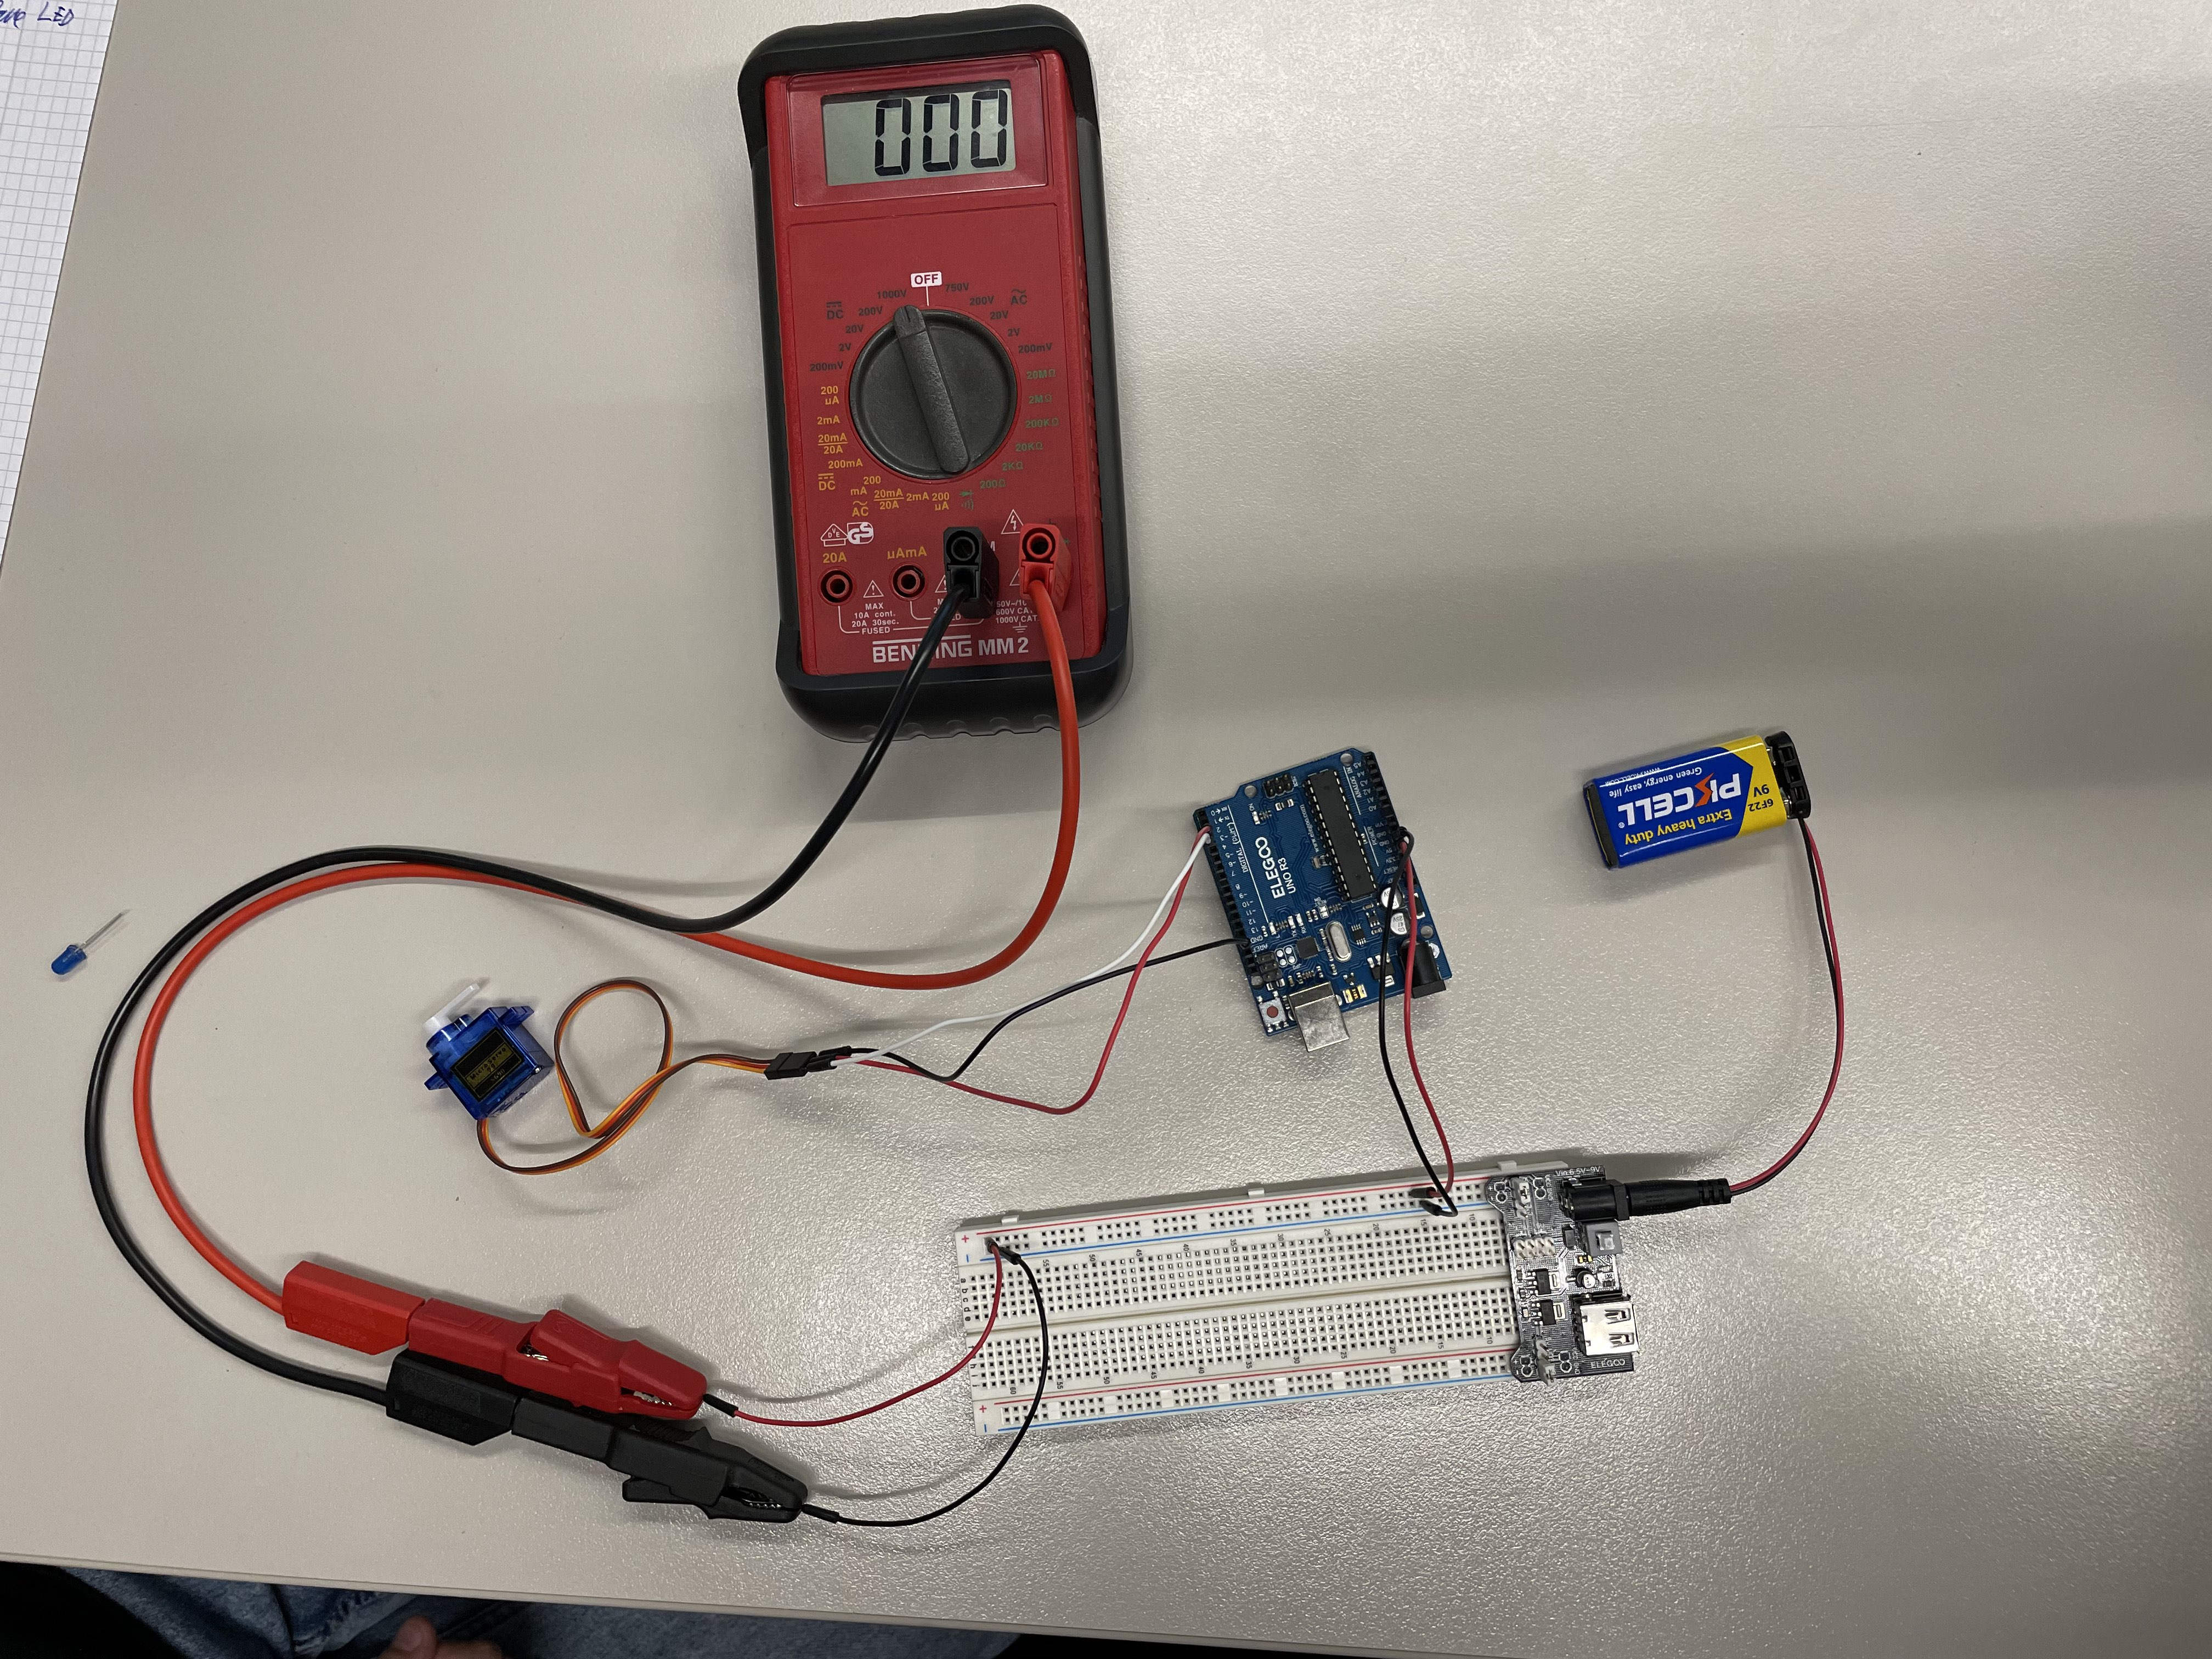
\includegraphics[width=9cm]{aufbau4}

\section{Messwerte}
\begin{center}
\begin{tabular}{ |c|c|c|c|c| }
  Messgröße & ohne Baugruppen & mit roter LED & mit blauer LED & mit Servomotor \\
  \hline
  Spannung [V] & 4.86 & 4.89 & 4.89 & 4.62 \\
  \hline
  Stromstärke [mA] & 34.1 & 39.0 & 37.5 & ? \\
  \hline
  Leistung rechn. [mW] & 165.726 & 190.71 & 183.375 & ? \\
  \hline
\end{tabular}
\end{center}

Die Leistung wurde errechnet, indem man die Spannung und die Stromstärke multipliziert:

\[ P = U * I \]

\section{Evtl. Beobachtungen}
Bei jedem Aufbau schwanken die Werte sehr, wodurch man warten muss, bis diese sich halbwegs stabilisieren. Das liegt wahrscheinlich an verschiedenen Bauteilen, wie Kondensatoren.

\section{Auswertung}
Man kann also sehen, dass die rote LED mehr Leistung braucht als die blaue LED und generell jeder Verbraucher mehr verbraucht als der Leerlauf ohne sämtliche Gruppen.

Testweise haben wir auch den ATmega328p in den "Power-down" deep sleep Modus gebracht, um den Stromverbrauch von ihm zu senken. Wir konnten aber keine messbare Änderung in der Leistung sehen, die über das normale Schwanken hinausging, was darauf hindeutet, dass der ATmega328p im Betrieb ohne jegliche andere Hardware sehr viel effizienter sein sollte.

Als grobe Schätzung kann eine Autobatterie 1kWh speichern, also 1000 Stunden lang 1W abgeben. Somit könnte ein Arduino UNO im Leerlauf mehr als 250 Tage am Stück laufen.

\end{document}
